\documentclass[11pt]{article}
\usepackage[margin=1in]{geometry}
\usepackage[T1]{fontenc}
\usepackage{lmodern,microtype}
\usepackage{amsmath,amssymb,amsthm,mathtools}
\usepackage{booktabs,longtable,array,enumitem}
\usepackage[numbers,sort&compress]{natbib}
\usepackage{pgfplots}
\pgfplotsset{compat=1.18}
\usepackage{listings}
\usepackage[hidelinks]{hyperref}
\usepackage{fancyhdr}
\pagestyle{fancy}\fancyhf{}
\fancyhead[L]{\small Hidden Slow Learners}\fancyhead[R]{\small Research companion v1.0}
\fancyfoot[C]{\thepage}
\setlength{\headheight}{14pt}
\setlength{\emergencystretch}{3em}
\setlength{\parskip}{4pt}
\newtheorem{theorem}{Theorem}[section]
\newtheorem{proposition}[theorem]{Proposition}
\newtheorem{lemma}[theorem]{Lemma}
\newtheorem{corollary}[theorem]{Corollary}
\theoremstyle{remark}\newtheorem{remark}[theorem]{Remark}
\newcommand{\R}{\mathbb{R}}
\newcommand{\E}{\mathbb{E}}
\newcommand{\Prob}{\mathbb{P}}
\newcommand{\rhoo}{\rho}
\newcommand{\ee}{\varepsilon}
\newcommand{\qsum}{Q}
\newcommand{\floorate}{\underline\eta}
\lstset{basicstyle=\ttfamily\footnotesize,breaklines=true,columns=fullflexible,frame=single,showstringspaces=false}
\title{\textbf{Hidden Slow Learners}\\[5pt]\large Finite-Horizon Limits and Rate-Aware Certificates\\for Adaptive-Market Stability}
\author{}
\date{18 September 2026\\[3pt]\small A reproducible companion to \emph{From Human Markets to Machine Markets}}
\begin{document}
\maketitle
\begin{abstract}
Can a short stress test distinguish a stable adaptive market from an unstable one? We study this question in a fixed positive linear market with heterogeneous exponentially updating decision states. An exact construction gives, for every finite response horizon, a stable and an unstable model with identical initial price-response coefficients, identical direct price persistence, and the same number of active adaptive agents. Their different hidden distributions of learning responses place total feedback on opposite sides of the stability boundary. The construction specializes classical interpolation and truncated-moment ideas; global priority for this application is not established. A valid external lower bound on learning rates yields conservative finite-horizon bounds on total feedback and a three-way stability diagnostic. Under explicitly assumed controlled kernel measurements with known Gaussian noise, simultaneous confidence across four declared horizons bounds the probability of any incorrect confident label. We execute 112 rationally constructed pairs, 336 common-shock comparisons, and 21,600 noisy measurement datasets across 108 synthetic configurations. All exact pairs have opposite stability. The rate-aware diagnostic makes no incorrect confident decision in this run, while remaining inconclusive on a substantial fraction of cases. A misspecified learning-rate floor produces false reassurance, demonstrating the importance of the measurement contract. These results establish an auditable model-specific research artifact, not a validated financial crisis detector, a new general stability theorem, or an independently replicated empirical discovery.
\end{abstract}
\noindent\textbf{Keywords:} adaptive markets; finite-horizon identification; positive systems; heterogeneous learning rates; truncated moments; stability certification.\\
\textbf{Evidence status:} proofs and executed synthetic experiments; no observed-market data or trained AI-agent population.

\section{Introduction}
A financial forecasting system may influence the process it forecasts. This observation is not itself a new research gap. Adaptive-agent finance has already investigated the interaction of forecasting, updating, and market stability \citep{georges2021}; performative prediction provides a general formal treatment of decision-induced changes in the data-generating environment \citep{perdomo2020}. The useful next question is narrower: \emph{what can an observer actually infer about stability from a limited response window?}

The preceding project framework treats market and learning states jointly. Its original numerical checks verify special-case algebra, but do not establish that the relevant feedback can be recovered from financially accessible measurements. This companion addresses that measurement gap through one deliberately small model. It asks whether short input--output observations can conceal different long-run learning feedback, and which additional information supports a defensible decision.

The intuition is simple. A slowly updating state can produce very little visible response per step while contributing substantial cumulative feedback over many steps. Matching the early response therefore need not match the total response. The mathematical challenge is stronger than showing two approximately similar plots: construct \emph{exactly identical finite response sequences} on opposite sides of a stability boundary, and then state precisely which additional assumptions can recover useful bounds.

Three contributions are developed. First, an explicit rational construction produces opposite-stability models with the same early kernel moments and hence the same early price responses. Second, a measurement contract combines a valid learning-rate floor with conservative bounds and an inconclusive outcome. Third, a reproducible experiment compares that diagnostic with truncation, a homogeneous-rate approximation, a simple matrix-pencil fit, and an oracle, while exposing a failure case under incorrect architectural information.

The ambition is a rigorous building block for the larger autonomous-market research program. The present result does not distinguish humans from AI: an equivalent hidden-memory mechanism could arise in human adaptive expectations or other positive dynamical systems. Nor does it show that conventional liquidity or leverage explanations fail empirically; those mechanisms are held absent here. Its claim is an identification limit in a specified model and a transparent way to avoid unwarranted certainty under a stronger information set.

\section{Related work and the novelty boundary}
\subsection{Feedback between forecasting and outcomes}
\citet{georges2021} already examine market stability with machine-learning agents. The accessible April 2019 author preprint, rather than an assumed identical final journal text, informed this audit. \citet{perdomo2020} develop performative prediction and conditions for convergence of retraining. More recent work studies stability of online algorithms under performative feedback \citep{farina2026}. These lines make it inappropriate to present ``models change markets and then learn from those markets'' as an original discovery. Our restricted question concerns finite input--output distinguishability, not a new equilibrium or regret concept.

\subsection{Positive systems and realization}
Positive-system theory supplies powerful stability and gain tools \citep{rantzer2015}. The threshold proved below is a direct specialization of that established mathematics. System identification already studies the estimation of Markov parameters and recovery of a state-space realization from sufficiently informative observations \citep{oymak2019}. Positivity-constrained identification is also established \citep{umenberger2016}. The present indistinguishability construction does not contradict finite-order recovery when enough well-conditioned data and valid order information are available. A method constrained in advance to stable realizations is not, by itself, evidence that an unknown underlying system is stable.

\subsection{Truncated moments}
Our kernel is a positive mixture of geometric sequences, so finite observations define a truncated moment problem. Parametrizing the possible measures consistent with finite moments is established mathematical territory \citep{fritzsche2020}. The signed barycentric construction below uses standard polynomial interpolation and partial-fraction identities. Its proposed contribution is the explicit adaptive-market stable/unstable pairing, equal active-agent count, measurement interpretation, and reproducible diagnostic benchmark. It is \emph{not} a claim to have invented moment ambiguity or positive-system stability.

\subsection{What has and has not been verified}
The literature audit checked primary records, abstracts, and selected accessible full texts as of 18 September 2026. It was focused rather than systematic. It did not establish absence of an equivalent construction in positive realization, identification, or heterogeneous-agent finance. The institutional motivation is consistent with concerns about AI-related correlated behavior and information gaps \citep{fsb2024}; that report does not validate this diagnostic. Global novelty, publication priority, and financial usefulness remain separate questions for external review. The repository includes the audit and a claim-by-claim evidence ledger.

\section{A restricted adaptive-market model}\label{sec:model}
Let $x_t\in\R$ denote a scalar deviation of price from an externally fixed reference. Agent $i$ maintains a signed price-pressure state $y_{i,t}$. For fixed parameters,
\begin{align}
 x_{t+1}&=a x_t+\sum_{i=1}^{n} y_{i,t}+\ee_{t+1},\label{eq:market}\\
 y_{i,t+1}&=(1-\eta_i)y_{i,t}+\eta_i q_i x_t.\label{eq:learn}
\end{align}
Assume $0\le a<1$, $q_i\ge0$, and $0<\eta_i\le1$. Write $r_i=1-\eta_i\in[0,1)$ and $Q=\sum_iq_i$. The linear state transition is
\begin{equation}
 J=\begin{pmatrix}
 a&\mathbf1^{\mathsf T}\\
 \operatorname{diag}(\eta)q&\operatorname{diag}(r)
 \end{pmatrix}.\label{eq:J}
\end{equation}
The state can be negative; ``positive'' means that the transition matrix is entrywise nonnegative. Stability throughout this paper means \emph{Schur stability}: $\rho(J)<1$. It is not a probability of a financial crisis.

The interpretation is an exponentially updated trend-following or forecast-pressure state. The term $q_i$ includes response sensitivity and normalized constant price impact. This is not a utility-maximizing trading model, a balance-sheet model, an inventory-conserving exchange, or an implementation of a trained neural agent. Parameters do not retrain or switch during a run. The simplicity is intentional: it permits exact identification statements before more realistic economics is introduced.

\begin{lemma}[Positive-feedback threshold]\label{lem:threshold}
Under the stated assumptions, $\rho(J)<1$ if and only if $a+Q<1$. Equality $a+Q=1$ implies $\rho(J)=1$; $a+Q>1$ implies $\rho(J)>1$.
\end{lemma}
\begin{proof}
Agents with $q_i=0$ add only eigenvalues $r_i<1$ and can be separated from the active subsystem. If there are no active agents, the claim follows from triangularity. Otherwise, the active matrix is irreducible and nonnegative. For $\lambda>\max_i r_i$, an eigenvector with first coordinate one has $i$th adaptive coordinate $\eta_iq_i/(\lambda-r_i)$. Its first equation is
\begin{equation}
 f(\lambda):=\lambda-a-\sum_i\frac{\eta_iq_i}{\lambda-r_i}=0.
\end{equation}
The function is strictly increasing on this interval, tends to $-\infty$ at the largest active pole, and tends to $+\infty$ at infinity. Its unique root has a strictly positive eigenvector and is the Perron eigenvalue. Since $f(1)=1-a-Q$, the location of that root relative to one yields all three statements. Passive eigenvalues remain strictly below one.
\end{proof}
\begin{remark}
Learning rates affect growth and decay times, although they cancel from this fixed positive-model threshold. No assertion follows for signed feedback, changing parameters, or nonlinear market impact. A negative-control example in Section~\ref{sec:failure} demonstrates the signed-feedback restriction.
\end{remark}

\section{Observable responses and hidden feedback}
Starting from $y_{i,0}=0$, eliminating the adaptive states gives
\begin{equation}
 x_{t+1}=a x_t+\sum_{j=0}^{t-1}k_jx_{t-1-j}+\ee_{t+1},\qquad
 k_j=\sum_iq_i(1-r_i)r_i^j.\label{eq:kernel}
\end{equation}
The infinite sum exists even when the closed-loop market is unstable:
\begin{equation}
 \sum_{j=0}^{\infty}k_j=\sum_iq_i=Q.\label{eq:Q}
\end{equation}
It is the \emph{open-loop memory kernel}, not the potentially diverging closed-loop impulse response, that is being summed.

Define $h_t$ by $x_0=1$, zero adaptive initial states, and no subsequent shock. Then $h_0=1$, $h_1=a$, and
\begin{equation}
 h_{t+1}=a h_t+\sum_{j=0}^{t-1}k_jh_{t-1-j}.\label{eq:impulse}
\end{equation}
Thus $k_0,\ldots,k_{K-1}$ determine $h_0,\ldots,h_{K+1}$. Conversely, with exact $a$ and exact impulse coefficients, a triangular recursion recovers those kernel terms; for example, $k_0=h_2-a^2$ and
\begin{equation}
 k_j=h_{j+2}-a h_{j+1}-\sum_{\ell=0}^{j-1}k_\ell h_{j-\ell}.
\end{equation}
This algebraic identity does not imply a benign noise model for deconvolved financial observations. Noise becomes dependent and can be amplified. The later Gaussian experiment therefore uses a separately stated controlled-measurement contract.

\section{Exact finite-horizon ambiguity}\label{sec:theorem}
\begin{theorem}[Opposite stability with identical finite responses]\label{thm:pair}
Fix $a\in[0,1)$ and a positive integer $K$. For any distinct ordered nodes $0\le r_0<\cdots<r_K<1$, there are two models satisfying Section~\ref{sec:model}, denoted $-$ and $+$, such that
\begin{align}
 a+Q_-&<1<a+Q_+,\label{eq:opposite}\\
 k_j^-&=k_j^+\quad(0\le j<K),\label{eq:matchk}\\
 h_t^-&=h_t^+\quad(0\le t\le K+1).\label{eq:matchh}
\end{align}
They can each be represented with exactly $K+1$ active agents, the same direct persistence $a$, and the same constant price-impact normalization. All parameters are rational when $a$ and the nodes are rational. Moreover, the first unmatched price coefficient differs strictly: $h_{K+2}^+-h_{K+2}^-=s>0$, with $s$ specified in the proof.
\end{theorem}
\begin{proof}
Let
\begin{equation}
 w_i=\frac{1}{\prod_{\ell\ne i}(r_i-r_\ell)}.
\end{equation}
Polynomial interpolation gives
\begin{equation}
 \sum_{i=0}^K w_i r_i^j=0\ (0\le j<K),\qquad
 \sum_{i=0}^K w_i r_i^K=1.\label{eq:moments}
\end{equation}
For completeness, interpolate the polynomial $z^j$ at the $K+1$ nodes and compare the coefficient of $z^K$. The coefficient vanishes for $j<K$ and equals one for $j=K$.

The partial-fraction identity
\begin{equation}
 \frac1{\prod_{i=0}^K(z-r_i)}=\sum_{i=0}^K\frac{w_i}{z-r_i}
\end{equation}
can be checked by matching residues and behavior at infinity. Evaluating at $z=1$ yields
\begin{equation}
 \sum_i\frac{w_i}{1-r_i}=\frac1{\prod_i(1-r_i)}>0.\label{eq:massgap}
\end{equation}
The signs of $w_i$ alternate, so both positive and negative parts are nonempty for $K\ge1$. Define
\begin{equation}
 B_+=\sum_i\frac{\max(w_i,0)}{1-r_i},\qquad
 B_-=\sum_i\frac{\max(-w_i,0)}{1-r_i},\qquad
 s=\frac{2(1-a)}{B_++B_-}.
\end{equation}
By \eqref{eq:massgap}, $B_+>B_->0$. Set
\begin{equation}
 q_i^+=\frac{s\max(w_i,0)}{1-r_i},\qquad
 q_i^-=\frac{s\max(-w_i,0)}{1-r_i},\qquad \eta_i=1-r_i.
\end{equation}
Their feedback totals are $Q_+=sB_+$ and $Q_-=sB_-$. The midpoint is $1-a$, hence \eqref{eq:opposite} follows, and Lemma~\ref{lem:threshold} establishes opposite stability. Their kernel difference equals $s\sum_iw_ir_i^j$, proving \eqref{eq:matchk}. Recursion \eqref{eq:impulse} proves \eqref{eq:matchh}; the first unmatched term has coefficient $h_0=1$, so its difference is $s$.

Remove zero-weight agents in each model. Each remaining positive $q_i$ may be divided among any number of identical-rate copies whose weights sum to $q_i$. Splitting until each model has $K+1$ active agents preserves its kernel and adds only stable difference modes with eigenvalues $r_i$. This gives the equal-count representation. Rationality follows from the construction.
\end{proof}

\begin{corollary}[No universally correct forced finite-window classifier]\label{cor:class}
For the pair in Theorem~\ref{thm:pair}, observations consisting of the declared finite impulse window cannot identify the stability label. With equal prior probability on the two members, any forced classifier using only that window has error probability $1/2$, including a randomized classifier. The conclusion also holds for any common finite input sequence whose response uses only the matched coefficients.
\end{corollary}
\begin{proof}
The observed deterministic vectors are identical. If a randomized rule returns stable with probability $p$ on this common vector, its average error is $\tfrac12(1-p)+\tfrac12p=\tfrac12$. Linearity gives the response to a common input as a convolution with $h$; over the stated window these convolutions coincide. Adding identically distributed observation noise preserves equality of the observation laws.
\end{proof}

The corollary permits an honest inconclusive answer. It does not state that every real market is unidentifiable, that more observations never help, or that a known low-order system remains unidentifiable after its relevant Markov parameters are observed. The order of our constructed family grows with the horizon. Nor does it compare stationary distributions: the unstable member generally has no ordinary stationary distribution under persistent shocks.

A floor $\eta_i\ge\floorate>0$ can be imposed by choosing all nodes below $1-\floorate$, provided $\floorate<1$. The construction still works for each finite $K$, though the resulting stability separation can become small. Thus a rate floor alone does not guarantee a uniformly decisive finite horizon arbitrarily close to the boundary. The floor is useful for bounds, not magic recovery.

\section{An exact, readable witness}\label{sec:witness}
Take $a=2/5$, $K=2$, and nodes $(0,1/2,19/20)$. Before equal-count splitting,
\begin{equation}
 q^-=(0,12/65,0),\qquad q^+=(54/1235,0,240/247),
 \qquad \eta=(1,1/2,1/20).
\end{equation}
Then $Q_-=12/65$ and $Q_+=66/65$. The stable model's active weight can be split into three identical-rate agents; one positive-model weight can be split once to give three active agents there as well. Equal numbers of active agents do not imply equal numbers of distinct learning rates.
\begin{table}[ht]
\centering\small
\begin{tabular}{lrr}
\toprule Quantity&Stable member&Unstable member\\\midrule
Direct price persistence $a$&0.400000&0.400000\\
Total hidden feedback $Q$&0.184615&1.015385\\
$a+Q$&0.584615&1.415385\\
Spectral radius $\rho(J)$&0.757909&1.032345\\
$h_0$&1.000000&1.000000\\
$h_1$&0.400000&0.400000\\
$h_2$&0.252308&0.252308\\
$h_3$&0.184000&0.184000\\
$h_4$&0.138428&0.159198\\\bottomrule
\end{tabular}
\caption{Exact rational witness, with decimal values rounded for display. The first four coefficients coincide exactly; the first nonzero difference is $h_4^+-h_4^-=27/1300$.}
\end{table}
The unstable model initially appears to recover from the unit shock. Its eventual dominant mode grows with an asymptotic e-folding time of approximately 31.41 model steps. These are not calibrated days or seconds. A homogeneous two-tap fit returns $Q=12/65$ for both models and therefore falsely labels the unstable one stable.

\begin{figure}[ht]
\centering
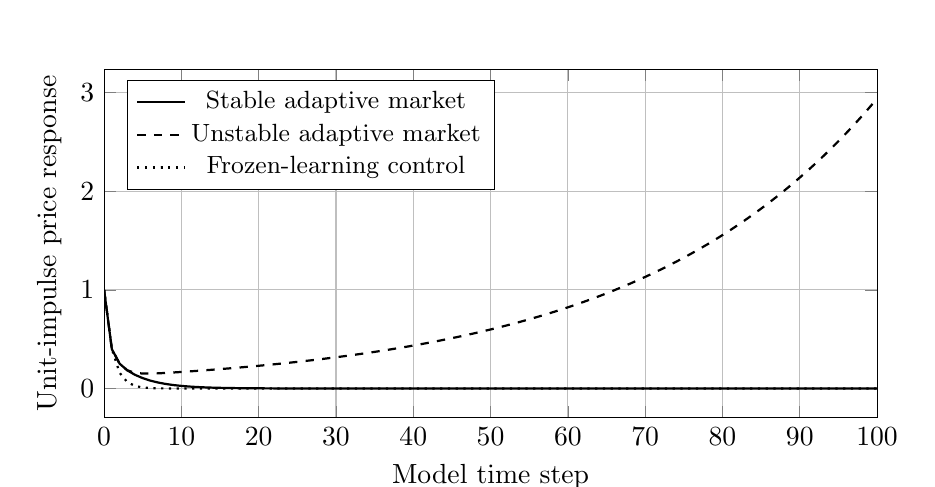
\begin{tikzpicture}
\begin{axis}[width=.94\linewidth,height=6cm,xlabel={Model time step},ylabel={Unit-impulse price response},legend pos=north west,legend style={font=\small},xmin=0,xmax=100,grid=major]
\addplot[thick] coordinates {(0,1) (1,0.4) (2,0.252307692308) (3,0.184) (4,0.138428402367) (5,0.104770177515) (6,0.0793854856623) (7,0.0601639949021) (8,0.0455983892637) (9,0.0345593508863) (10,0.0261928200308) (11,0.0198517617784) (12,0.0150458203665) (13,0.0114033562922) (14,0.00864270154657) (15,0.00655037763737) (16,0.00496458739939) (17,0.00376270337542) (18,0.0028517851641) (19,0.00216139243803) (20,0.00163813786886) (21,0.0012415587425) (22,0.000940988020831) (23,0.000713182892633) (24,0.000540527431895) (25,0.000409670377191) (26,0.00031049269296) (27,0.000235325075352) (28,0.00017835489319) (29,0.000135176703448) (30,0.000102451583068) (31,7.76489336204e-05) (32,5.8850792851e-05) (33,4.46035207145e-05) (34,3.38053909514e-05) (35,2.56213957793e-05) (36,1.94186756374e-05) (37,1.47175808359e-05) (38,1.11545807606e-05) (39,8.45415244065e-06) (40,6.40747465314e-06) (41,4.85628000191e-06) (42,3.68061626984e-06) (43,2.78957064265e-06) (44,2.11423951856e-06) (45,1.60240026672e-06) (46,1.21447290728e-06) (47,9.20459433985e-07) (48,6.97624100571e-07) (49,5.28735289931e-07) (50,4.00733011646e-07) (51,3.0371898695e-07) (52,2.30191225463e-07) (53,1.74463904322e-07) (54,1.32227689609e-07) (55,1.00216500183e-07) (56,7.59549451295e-08) (57,5.75669044431e-08) (58,4.36304506771e-08) (59,3.30678928232e-08) (60,2.50624396218e-08) (61,1.8995037971e-08) (62,1.43965022146e-08) (63,1.09112325194e-08) (64,8.26971672123e-09) (65,6.26768923933e-09) (66,4.75033543773e-09) (67,3.60031997587e-09) (68,2.72871339268e-09) (69,2.06811528678e-09) (70,1.56744231582e-09) (71,1.18797797643e-09) (72,9.0037869862e-10) (73,6.82404738989e-10) (74,5.17200405238e-10) (75,3.91990623593e-10) (76,2.97093056054e-10) (77,2.251693756e-10) (78,1.70657801234e-10) (79,1.29343011431e-10) (80,9.80301778471e-11) (81,7.42979126776e-11) (82,5.6311025334e-11) (83,4.26786091276e-11) (84,3.23464839481e-11) (85,2.45156776472e-11) (86,1.85806423804e-11) (87,1.40824282419e-11) (88,1.06731931614e-11) (89,8.08930464994e-12) (90,6.13095338295e-12) (91,4.64670215928e-12) (92,3.52177542519e-12) (93,2.66918380398e-12) (94,2.02299730087e-12) (95,1.53324700728e-12) (96,1.16206105876e-12) (97,8.8073604441e-13) (98,6.67517402872e-13) (99,5.05917165494e-13) (100,3.83438959405e-13)};\addlegendentry{Stable adaptive market}
\addplot[thick,dashed] coordinates {(0,1) (1,0.4) (2,0.252307692308) (3,0.184) (4,0.159197633136) (5,0.151500946746) (6,0.151083266727) (7,0.153763928334) (8,0.157822693343) (9,0.162548170167) (10,0.167648537848) (11,0.173005956031) (12,0.178574844993) (13,0.184339695664) (14,0.190297578644) (15,0.196450894394) (16,0.202804370525) (17,0.209363820401) (18,0.216135632254) (19,0.223126561359) (20,0.230343648016) (21,0.237794187829) (22,0.245485723822) (23,0.253426047744) (24,0.261623205337) (25,0.270085503403) (26,0.278821517768) (27,0.287840101786) (28,0.297150395235) (29,0.306761833546) (30,0.316684157353) (31,0.326927422358) (32,0.337502009521) (33,0.348418635577) (34,0.3596883639) (35,0.371322615711) (36,0.383333181656) (37,0.395732233754) (38,0.408532337731) (39,0.421746465757) (40,0.435388009592) (41,0.449470794157) (42,0.464009091544) (43,0.479017635482) (44,0.494511636268) (45,0.510506796183) (46,0.5270193254) (47,0.54406595842) (48,0.561663971026) (49,0.579831197792) (50,0.598586050159) (51,0.617947535092) (52,0.637935274344) (53,0.658569524338) (54,0.679871196703) (55,0.701861879459) (56,0.7245638589) (57,0.748000142177) (58,0.772194480616) (59,0.797171393789) (60,0.822956194363) (61,0.849575013752) (62,0.877054828598) (63,0.905423488116) (64,0.934709742312) (65,0.964943271121) (66,0.996154714489) (67,1.02837570342) (68,1.06163889203) (69,1.09597799066) (70,1.1314278) (71,1.1680242464) (72,1.20580441826) (73,1.24480660361) (74,1.28507032892) (75,1.32663639917) (76,1.36954693918) (77,1.41384543632) (78,1.45957678456) (79,1.50678733) (80,1.55552491782) (81,1.60583894076) (82,1.65778038919) (83,1.71140190279) (84,1.76675782387) (85,1.82390425249) (86,1.88289910326) (87,1.94380216408) (88,2.0066751567) (89,2.07158179928) (90,2.13858787098) (91,2.20776127859) (92,2.2791721254) (93,2.3528927822) (94,2.42899796063) (95,2.50756478891) (96,2.58867289002) (97,2.67240446235) (98,2.75884436305) (99,2.84808019397) (100,2.94020239052)};\addlegendentry{Unstable adaptive market}
\addplot[thick,dotted] coordinates {(0,1) (1,0.4) (2,0.16) (3,0.064) (4,0.0256) (5,0.01024) (6,0.004096) (7,0.0016384) (8,0.00065536) (9,0.000262144) (10,0.0001048576) (11,4.194304e-05) (12,1.6777216e-05) (13,6.7108864e-06) (14,2.68435456e-06) (15,1.073741824e-06) (16,4.294967296e-07) (17,1.7179869184e-07) (18,6.8719476736e-08) (19,2.74877906944e-08) (20,1.09951162778e-08) (21,4.3980465111e-09) (22,1.75921860444e-09) (23,7.03687441777e-10) (24,2.81474976711e-10) (25,1.12589990684e-10) (26,4.50359962737e-11) (27,1.80143985095e-11) (28,7.20575940379e-12) (29,2.88230376152e-12) (30,1.15292150461e-12) (31,4.61168601843e-13) (32,1.84467440737e-13) (33,7.37869762948e-14) (34,2.95147905179e-14) (35,1.18059162072e-14) (36,4.72236648287e-15) (37,1.88894659315e-15) (38,7.55578637259e-16) (39,3.02231454904e-16) (40,1.20892581961e-16) (41,4.83570327846e-17) (42,1.93428131138e-17) (43,7.73712524553e-18) (44,3.09485009821e-18) (45,1.23794003929e-18) (46,4.95176015714e-19) (47,1.98070406286e-19) (48,7.92281625143e-20) (49,3.16912650057e-20) (50,1.26765060023e-20) (51,5.07060240091e-21) (52,2.02824096037e-21) (53,8.11296384146e-22) (54,3.24518553658e-22) (55,1.29807421463e-22) (56,5.19229685853e-23) (57,2.07691874341e-23) (58,8.30767497366e-24) (59,3.32306998946e-24) (60,1.32922799578e-24) (61,5.31691198314e-25) (62,2.12676479326e-25) (63,8.50705917302e-26) (64,3.40282366921e-26) (65,1.36112946768e-26) (66,5.44451787074e-27) (67,2.17780714829e-27) (68,8.71122859318e-28) (69,3.48449143727e-28) (70,1.39379657491e-28) (71,5.57518629963e-29) (72,2.23007451985e-29) (73,8.92029807941e-30) (74,3.56811923176e-30) (75,1.42724769271e-30) (76,5.70899077082e-31) (77,2.28359630833e-31) (78,9.13438523332e-32) (79,3.65375409333e-32) (80,1.46150163733e-32) (81,5.84600654932e-33) (82,2.33840261973e-33) (83,9.35361047892e-34) (84,3.74144419157e-34) (85,1.49657767663e-34) (86,5.98631070651e-35) (87,2.3945242826e-35) (88,9.57809713041e-36) (89,3.83123885216e-36) (90,1.53249554087e-36) (91,6.12998216346e-37) (92,2.45199286539e-37) (93,9.80797146154e-38) (94,3.92318858462e-38) (95,1.56927543385e-38) (96,6.27710173539e-39) (97,2.51084069415e-39) (98,1.00433627766e-39) (99,4.01734511065e-40) (100,1.60693804426e-40)};\addlegendentry{Frozen-learning control}
\end{axis}
\end{tikzpicture}
\caption{Executed witness trajectories. Frozen learning has zero adaptive state and follows $a^t$; it is a mechanism control, not a matched observational explanation. All coordinates are embedded in this source.}
\end{figure}

\begin{proposition}[Why a one-rate fit can give false reassurance]\label{prop:jensen}
If $k_0>0$, the homogeneous-rate extrapolation satisfies
\begin{equation}
 \widehat Q_{\mathrm{one}}=\frac{k_0^2}{k_0-k_1}\le Q.
\end{equation}
Equality holds when all active agents have the same rate. For heterogeneous active rates, the inequality is strict.
\end{proposition}
\begin{proof}
Let $p_i=q_i(1-r_i)/k_0$, so $\sum p_i=1$ and $\sum p_ir_i=k_1/k_0$. Since $z\mapsto1/(1-z)$ is strictly convex on $[0,1)$,
\begin{equation}
 Q=k_0\sum_i\frac{p_i}{1-r_i}
 \ge\frac{k_0}{1-\sum_i p_ir_i}=\frac{k_0^2}{k_0-k_1}.
\end{equation}
Strictness follows from strict convexity when at least two active rates differ.
\end{proof}
This lower bound can support an instability declaration with exact data if it already exceeds $1-a$. Its being below that boundary does not certify stability. This analytic explanation was documented with the result; it was not used to tune the fixed noisy experiment or to construct an improved competing interval estimator.

\section{Rate-aware outer bounds}\label{sec:bounds}
Suppose a valid architectural statement guarantees $\eta_i\ge\floorate>0$ for every relevant active state. Let $\bar r=1-\floorate$ and $S_H=\sum_{j=0}^{H-1}k_j$ for $H\ge1$.
\begin{proposition}[Finite-horizon feedback bounds]\label{prop:bounds}
Under the model and valid floor,
\begin{equation}
 S_H\le Q\le U_H:=\min\left\{
 \frac{S_H}{1-\bar r^H},\quad
 S_H+\frac{\bar r}{\floorate}k_{H-1}\right\}.\label{eq:bounds}
\end{equation}
These are outer bounds; they need not be optimal given the full observed moment sequence.
\end{proposition}
\begin{proof}
Finite geometric summation gives
\begin{equation}
 S_H=\sum_iq_i(1-r_i^H),\qquad Q-S_H=\sum_iq_ir_i^H.
\end{equation}
Nonnegativity yields $S_H\le Q$, and $1-r_i^H\ge1-\bar r^H$ yields the first upper bound. For the second,
\begin{equation}
 \sum_iq_ir_i^H
 =\sum_iq_i(1-r_i)r_i^{H-1}\frac{r_i}{1-r_i}
 \le\frac{\bar r}{\floorate}k_{H-1}.
\end{equation}
The case $\floorate=1$ has $r_i=0$ and $Q=S_H$ for every $H\ge1$.
\end{proof}
If all active rates equal the floor, both upper bounds equal $Q$; if rates are faster, the bounds can be loose. For exact observations, label stable when $a+U_H<1$, unstable when $a+S_H>1$, and inconclusive otherwise. The noiseless interval contracts as the accumulated response reveals the tail, but no finite-horizon uniform margin guarantee is assumed. A simple uniform tail requirement is $Q\bar r^H\le\delta$, requiring a horizon that grows as the rate floor becomes small.

Without a floor, our conservative implementation uses the valid lower bound $S_H$ and upper bound $+\infty$. It can then identify instability but never stability. This is an intentionally simple procedure, not a claim that every possible exact moment vector permits arbitrarily large feedback; special moment sequences or additional order restrictions can identify more.

\section{Measurement contract and statistical guarantee}\label{sec:measurement}
\subsection{Two different information sets}
The impossibility result uses only finite \emph{closed-loop price responses}. The diagnostic experiment instead assumes \emph{controlled loop-open kernel measurements} in a trusted shadow replay. For each replay, set all adaptive states to zero, present one unit of market input, clamp subsequent market inputs to zero while allowing the adaptive memories to decay, and record their aggregate price pressure. This produces the sequence $k_0,k_1,\ldots$ without closing the price-feedback loop. The main simulator verifies equality between this agent-level replay and the analytical kernel.

Such access is plausible as a proposed laboratory interface but is not shown available at financial-system scale. The controller must isolate input from resulting feedback, observe aggregate response in consistent units, and audit the minimum active learning rate. A black-box stock-price series does not automatically supply any of these. Unknown $a$, changes of units, model drift, omitted adaptive states, or endogenous measurement noise require a different inference analysis.

\subsection{Simultaneous Gaussian construction}
The executed experiment observes means
\begin{equation}
 \widehat k_j=k_j+Z_j,\quad Z_j\stackrel{\mathrm{ind}}\sim N(0,v^2),\quad
 v=\frac{\sigma}{\sqrt{R}},\ R=128,
\end{equation}
with known $v$. Four horizons $\mathcal H=\{4,16,64,256\}$ are declared in advance. Let $m=|\mathcal H|=4$, $\alpha=0.05$, and
\begin{equation}
 z=\Phi^{-1}\!\left(1-\frac{\alpha}{4m}\right).
\end{equation}
For each $H\in\mathcal H$, define
\begin{align}
 S_H^-&=\widehat S_H-zv\sqrt H,&
 S_H^+&=\widehat S_H+zv\sqrt H,&
 K_H^+&=\widehat k_{H-1}+zv,\\
 L_H&=\max(0,S_H^-),&
 \widetilde U_H&=\min\left\{\frac{S_H^+}{1-\bar r^H},
 S_H^++\frac{\bar r}{\floorate}K_H^+\right\}.\label{eq:ci}
\end{align}
Endpoints inconsistent with nonnegative moments, or a reversed interval, produce \texttt{model\_conflict}, not a stability label. Otherwise the rule returns stable if $a+\widetilde U_H<1$, unstable if $a+L_H>1$, and inconclusive otherwise. Numerical code uses a $10^{-12}$ boundary tolerance.

\begin{theorem}[Finite-family error guarantee]\label{thm:ci}
Under the fixed positive model, known $a$, a valid rate floor, and the stated independent Gaussian measurement errors, the probability that any of the four declared horizons produces an incorrect confident label is at most $\alpha$.
\end{theorem}
\begin{proof}
For each horizon, the partial-sum error is Gaussian with standard deviation $v\sqrt H$; the terminal-tap error has standard deviation $v$. There are $2m$ two-sided intervals. Each has failure probability $\alpha/(2m)$ by the chosen $z$. A union bound gives simultaneous coverage at least $1-\alpha$; it does not require independence between sums, terminal taps, or horizons. On that event, nonnegativity holds and Proposition~\ref{prop:bounds} gives $L_H\le Q\le\widetilde U_H$ at every horizon. Lemma~\ref{lem:threshold} then makes either strict confident decision correct. Hence an incorrect confident decision is contained in the complement of the simultaneous event.
\end{proof}
This is an \emph{unconditional finite-family} guarantee, not a bound on the conditional error among only decided cases. It is also not an anytime-valid statement for unlimited monitoring or a guarantee under a misspecified rate floor. Reusing these Gaussian endpoints on kernels deconvolved from noisy market prices would violate the measurement contract.

\section{Executed experimental design}\label{sec:design}
The numerical configuration is recorded in \texttt{configs/main.json}. It was fixed before the full run, after exploratory algebra and the readable witness were developed. This is not an externally registered preregistration. No market dataset, commercial API, GPU, pretrained model, or real-money transaction was used.

\subsection{Exact paired models}
The grid takes $K\in\{1,2,3,4,6,8,12\}$, $a\in\{1/5,2/5,3/5,4/5\}$, and terminal persistence in $\{0.9,0.99,0.999,0.9999\}$, giving 112 pairs. For $K>1$, the first $K$ nodes are evenly spaced from zero to $3/4$ and the final node is the chosen terminal persistence; for $K=1$ the first node is zero. Rational arithmetic generates the witnesses. Floating-point agent iteration and state-matrix responses provide separate numerical checks. Three common shock sequences per pair give 336 finite-path comparisons. The rational verifier independently checks identities without importing the main package.

\subsection{Noisy controlled-measurement panel}
The panel has $3\times3\times3\times4=108$ configurations: $a\in\{0.2,0.5,0.8\}$, rate floor in $\{0.002,0.02,0.1\}$, slow-feedback share in $\{0,0.3,0.7\}$, and total-feedback ratio $Q/(1-a)\in\{0.6,0.9,1.1,1.4\}$. Each configuration has eight state slots. Four slow rates are the floor times $(1,1.3,1.8,2.5)$; four fast rates are independently drawn uniformly from $[0.2,0.9]$. Dirichlet weights distribute each group's allocated $Q$. At slow share zero, the slow slots have zero feedback, so the floor is conservative and fewer states are active.

For each configuration, two observation-noise levels $\sigma/(1-a)\in\{0.002,0.02\}$ and 100 independent repetitions yield 21,600 datasets. Each dataset supplies the four horizons, giving 86,400 decision rows. The Gaussian sample means are drawn directly from their exact distribution for $R=128$ replicates. This is distribution-equivalent measurement simulation, \emph{not} 2.76 million separately executed market episodes. The first 32 noisy taps and the sums and terminal taps used at all horizons are archived; all 256 taps can be regenerated from recorded seeds.

\subsection{Comparators and their information}
\begin{table}[ht]
\centering\small
\begin{tabular}{p{.20\linewidth}p{.70\linewidth}}
\toprule Method&Definition and limitations\\\midrule
Rate-aware interval&Equation~\eqref{eq:ci}, known valid floor, known noise; can abstain.\\
No-floor interval&Same lower confidence bound; infinite upper bound; can identify instability only.\\
Truncated sum&Point estimate $\max(0,\widehat S_H)$; implicitly ignores the unobserved tail and measurement uncertainty.\\
One-rate fit&Two-tap geometric extrapolation; no heterogeneous-rate or noise certificate.\\
Matrix pencil&Conventional Hankel/SVD fit, maximum rank eight, fixed noise-aware cutoff, positivity and floor checks; at most 32 early taps.\\
Oracle&Uses the true hidden $Q$; extra information, not a feasible estimator.\\\bottomrule
\end{tabular}
\caption{This is a mechanism/ablation comparison, not a state-of-the-art benchmark.}
\end{table}
For the matrix pencil, a square Hankel block of size $p=\min(8,\lfloor H/2\rfloor)$ is used, after capping available taps at 32. Singular values below $\max(5vp,10^{-10}s_1)$ are discarded. Real retained roots must lie in $[0,1-\floorate]$ within tolerance, and fitted nonnegative amplitudes determine a geometric tail estimate. Invalid fits return inconclusive. At long horizons this comparator does \emph{not} use all information available to the rate-aware method; it is neither an optimized identification suite nor a faithful reproduction of every procedure in \citet{oymak2019}. Stronger full-horizon, positivity-constrained and moment-feasibility comparisons are required before any broad performance claim.

\section{Results}\label{sec:results}
\subsection{Exact equality and opposite stability}
All 112 pairs have opposite stability. The largest floating-point mismatch among matched price coefficients is $3.33\times10^{-16}$; among matched kernel coefficients it is $5.55\times10^{-17}$. All 336 common-shock path comparisons agree within $2.22\times10^{-15}$. The independent rational implementation verifies exact equality for all 112 pairs plus the separate readable witness. Exact rational proof is the primary basis for equality; floating-point tolerances are implementation checks.

Some pairs are near the boundary: the smallest unstable spectral-radius excess in the grid is approximately $9.12\times10^{-7}$. The study does not describe every pair as a rapidly exploding crisis. The readable witness has a larger unstable radius, approximately 1.032345, illustrating a visible delayed-feedback effect without claiming a calibration to actual markets.

\subsection{Coverage and false reassurance}
Across all 21,600 datasets and four horizons, the rate-aware procedure produces zero incorrect confident labels. It does not always decide. Table~\ref{tab:coverage} reports the fraction of all datasets receiving stable or unstable rather than an inconclusive/conflict outcome.
\begin{table}[ht]
\centering\small
\begin{tabular}{rrrrr}
\toprule &\multicolumn{2}{c}{Lower noise: $\sigma/(1-a)=0.002$}&\multicolumn{2}{c}{Higher noise: $0.02$}\\
$H$&Rate-aware&No floor&Rate-aware&No floor\\\midrule
4 & 23.15 & 14.81 & 22.87 & 14.54 \\
16 & 63.66 & 31.59 & 51.84 & 29.85 \\
64 & 78.43 & 39.75 & 62.49 & 37.35 \\
256 & 82.69 & 42.49 & 66.20 & 37.21 \\
\bottomrule
\end{tabular}
\caption{Decision coverage in percent; 10,800 datasets per noise condition. No-floor coverage reflects instability declarations only.}\label{tab:coverage}
\end{table}
Longer horizons reveal more feedback, but summing additional noisy taps also increases uncertainty. Consequently decision coverage need not rise monotonically under the fixed endpoint rule. The higher-noise no-floor procedure illustrates this trade-off between accumulated signal and sum variance.

\begin{table}[ht]
\centering\small
\begin{tabular}{rrrrr}
\toprule $H$&Rate-aware&Truncated sum&One-rate fit&Matrix pencil\\\midrule
4 & 0.00 & 70.37 & 66.67 & 39.26 \\
16 & 0.00 & 35.26 & 66.67 & 30.78 \\
64 & 0.00 & 20.37 & 66.67 & 29.87 \\
256 & 0.00 & 14.81 & 66.67 & 29.87 \\
\bottomrule
\end{tabular}
\caption{Lower-noise condition: percent of the 5,400 truly unstable datasets labeled \emph{stable}. This is false reassurance, not overall error or conditional-on-decision error. Rate-aware decision coverage is reported separately. The matrix pencil uses a 32-tap cap.}\label{tab:false}
\end{table}
The point-estimation baselines often return a label when the interval procedure declines to decide. Therefore zero errors must not be presented without coverage. At $H=256$ and lower noise, the rate-aware method decides on 82.69\% of datasets; the matrix pencil decides on 99.99\%. The observed false-stable fractions are 0\% and 29.87\%, respectively, under the stated, unequal long-horizon information use. Those results support caution about tail extrapolation in this panel, not universal dominance over system identification.

The simultaneous Gaussian measurement-interval event occurs in 95.29\% and 95.53\% of datasets for the two noise levels. Actual joint coverage of $Q$ by all derived outer intervals is 99.07\% and 98.81\%, respectively. Some intervals fail to cover or conflict off the simultaneous event, but none leads to an incorrect confident declaration in this run. All outcomes, including conflicts and nondecisions, remain in the archived rows.

An additional design-average error summary uses one indicator per independent dataset: whether \emph{any} horizon made an incorrect confident decision. With zero such indicators in 21,600 datasets, a conservative two-sided Hoeffding 95\% interval for the fixed-design average probability is $[0,0.00924]$. The four correlated horizons are not treated as 86,400 independent samples. This interval describes the stated synthetic design, not future market risk or the error conditional on selecting decisive cases.

\section{Failure tests and limits}\label{sec:failure}
\subsection{A false learning-rate floor can certify an unstable model}
Take $a=0.4$, $Q=0.8$, and a single true rate $\eta=0.001$. The model is unstable because $a+Q=1.2$. At $H=4$, exact observations and the correct floor give approximately
\begin{equation}
 Q\in[0.0031952,\ 0.8],
\end{equation}
so the answer is inconclusive. Incorrectly asserting a floor of $0.2$ produces upper bound approximately $0.00541193$, and therefore a false stable label. This is not a failure of the theorem under its assumptions: it is a concrete demonstration that the architectural contract must be audited. Extending this example to $H=2048$ reveals enough cumulative feedback to identify instability even from the lower bound alone.

\subsection{Signed feedback invalidates the positive threshold}
With $a=0.4$, $q=-1.5$, and $\eta=1$, the matrix
\begin{equation}
 \begin{pmatrix}0.4&1\\-1.5&0\end{pmatrix}
\end{equation}
has spectral radius $\sqrt{1.5}\approx1.224745$, despite $a+Q=-1.1<1$. The positivity assumption is violated. The public model implementation rejects negative $q$; the negative control explicitly constructs the out-of-class matrix. Signed stabilizing and destabilizing strategies need a more general analysis.

\subsection{Economic and statistical boundaries}
The fixed linear model omits solvency constraints, inventory accounting, collateral, strategic interaction, heterogeneous information, spreads, and endogenous liquidity. It neither estimates AI participation nor identifies a universal penetration threshold. The construction varies hidden learning responses, not solely the identity of a model provider. A human adaptive-expectations model can have the same equations.

The Gaussian measurement model assumes independent tap errors of known variance, exact $a$, and an externally valid minimum rate. In actual shadow experiments, correlated errors, state-reset failures, model changes, and omitted slow components could undermine the intervals. Robust confidence under dependent errors, uncertainty in $a$, and unknown support are unfinished research tasks. The current geometric bounds ignore information in many interior moments; optimized moment-feasibility intervals may decide more cases. No economic-loss or liquidity-preservation claim is made for abstention: the diagnostic abstains from \emph{labeling}, not from trading.

\section{Reproducibility and evidence accounting}\label{sec:repro}
The release contains exact witnesses, input-generating seeds, raw estimator inputs, every decision row, aggregate summaries, unit tests, and standalone verifiers. Twenty-nine tests passed in the delivered code version. A standard-library-only rational verifier checks all exact pairs and the readable example without importing the model package. A separately implemented measurement verifier regenerates all 21,600 noisy input datasets and recomputes all 86,400 rate-aware decisions without importing the main inference functions. A clean-output-directory rerun matches 17 data files: CSV/JSON byte-for-byte excluding environment metadata, and NPZ arrays element-for-element.

All these checks were executed in the same computational environment and authoring process. They establish internal reproducibility and reduce shared-code risk; they do not constitute replication by an independent researcher. The paper is self-contained for LaTeX compilation, while the companion folder is required to rerun the numerical study. No external bibliography or figure file is needed to compile this source.

The recorded full numerical run used Python 3.13.5, NumPy 2.3.5, and SciPy 1.17.0. Timing is stored as environment metadata rather than a general performance claim. Dependency constraints, the actual version lock, configuration, and exact commands are in the repository. A smoke mode checks functionality on a reduced design but is not a substitute for the full experiment.

\section{What would turn this into a larger contribution?}
The strongest next target is not a new name for feedback stability. It is evidence that the measurement distinction survives stronger alternatives and economic realism. First, a control/moment-theory expert should assess priority and verify the exact theorem independently. Second, a full-horizon constrained-identification or moment-feasibility method should compete under the same information and compute budgets. Third, a financially accounted market environment should test whether the hidden slow-feedback phenomenon persists with inventory, liquidity, solvency, and adaptive policies. Fourth, a real laboratory measurement protocol must establish whether the rate floor and kernel observations can be obtained without assuming away the difficult part.

A generalizable financial contribution would require an interpretable mechanism, measured incremental information beyond conventional explanations, robustness to architecture changes, and external reproduction. A globally useful stability framework would require much more: validated data access, calibrated economic consequences, and demonstrable decision value. None of those achievements is inferred from the present exact construction. Conversely, discovering that a stronger conventional estimator resolves the proposed cases would be valuable evidence, not a reason to hide the comparison.

\section{Conclusion}
Finite calm-looking responses are not, by themselves, a stability certificate in the stated heterogeneous adaptive-memory model. For every finite horizon, an exact construction places two observationally matched models on opposite sides of the stability boundary. A valid learning-rate floor and controlled kernel observations permit conservative decisions, but also require an explicit inconclusive outcome. The executed synthetic study supports the implementation and illustrates both benefits and assumptions; a wrong floor can create false reassurance. This is a concrete and reproducible candidate building block for the machine-market research program. Its global novelty, empirical financial importance, and independent external reproducibility remain to be established.

\appendix
\section{Implementation and reproduction commands}
From the extracted folder root:
\begin{lstlisting}
python3 -m venv .venv
source .venv/bin/activate
python -m pip install -r requirements.txt
python -m pytest -q
python scripts/run_experiments.py
python scripts/verify_exact.py
python scripts/verify_measurements.py
python scripts/build_figures.py
\end{lstlisting}
The exact verifier uses Python's \texttt{fractions.Fraction}. The measurement verifier reads the archived arrays once, regenerates noises from \texttt{SeedSequence}, and uses a separately coded confidence calculation. These two verifiers should be inspected, not accepted solely because they print PASS. On Windows, use the environment activation command documented in the README.

Compile this file twice with \texttt{pdflatex -interaction=nonstopmode -halt-on-error Hidden\_Slow\_Learners.tex}. No shell escape is needed. To preserve delivered reference outputs while testing a new environment, use \texttt{--output reproduced\_results} and point both verifiers to that directory. The release also includes a manifest and an external-reproduction checklist.

\section{Data and comparison definitions}
The exact pair table records parameters, margins, radii, and numerical residuals; the witness JSON stores rational numbers as strings to avoid binary roundoff. \texttt{measurement\_inputs.npz} stores first-tap means, horizon sums, terminal taps, standard errors, case IDs, noise IDs, and repetition IDs. \texttt{configurations.json} records all hidden model parameters for auditing ground truth. \texttt{decisions.csv} stores one row for each dataset--horizon combination and all six method outputs.

``Decision coverage'' is the number of stable or unstable labels divided by all datasets in a stratum. ``False-stable fraction'' uses truly unstable datasets as its denominator, not all decisions. ``Unconditional error'' divides wrong confident labels by all datasets. A model-conflict outcome counts as no decision, not as a correct stable label. The full CSV retains false-unstable outcomes as well, including the small number produced by the matrix-pencil fit. The oracle is a ground-truth check and has privileged parameter access.

\section{Provenance and disclosure}
The original broad manuscript and concept note are retained unchanged under \texttt{provenance/}. They are historical inputs, not independently revalidated empirical claims. This companion develops a separate finite-horizon construction, proofs, measurement contract, code, and synthetic experiments during the requested research session. The focused web audit and mathematical derivation are distinct from the user's supplied outline.

The manuscript and code were developed with AI assistance in a computational session. A human researcher must verify authorship eligibility, contribution statements, disclosure requirements, licensing, references, and institutional or journal policies before public submission. No author name, affiliation, funding source, ethics approval, external replication, or real-data access has been invented. Any future claim of first discovery requires a deeper review of the neighboring mathematical and financial literatures.

\begin{thebibliography}{99}
\bibitem[Georges and Pereira(2021)]{georges2021}
C. Georges and J. Pereira. Market stability with machine learning agents. \emph{Journal of Economic Dynamics and Control}, 122:104032, 2021. \href{https://doi.org/10.1016/j.jedc.2020.104032}{doi:10.1016/j.jedc.2020.104032}. Accessible author preprint dated 18 April 2019: \url{https://academics.hamilton.edu/economics/cgeorges/risk-ml-april-2019.pdf}.
\bibitem[Perdomo et al.(2020)]{perdomo2020}
J. Perdomo, T. Zrnic, C. Mendler-D\"unner, and M. Hardt. Performative prediction. \emph{Proceedings of Machine Learning Research}, 119:7599--7609, 2020. \url{https://proceedings.mlr.press/v119/perdomo20a.html}.
\bibitem[Rantzer(2015)]{rantzer2015}
A. Rantzer. Scalable control of positive systems. \emph{European Journal of Control}, 24:72--80, 2015. \href{https://doi.org/10.1016/j.ejcon.2015.04.004}{doi:10.1016/j.ejcon.2015.04.004}.
\bibitem[Oymak and Ozay(2019)]{oymak2019}
S. Oymak and N. Ozay. Non-asymptotic identification of LTI systems from a single trajectory. arXiv:1806.05722v2, revised 3 February 2019. \url{https://arxiv.org/abs/1806.05722v2}. Preprint version consulted.
\bibitem[Umenberger and Manchester(2016)]{umenberger2016}
J. Umenberger and I. R. Manchester. Scalable identification of stable positive systems. In \emph{IEEE Conference on Decision and Control}, pp.\ 4630--4635, 2016. \href{https://doi.org/10.1109/CDC.2016.7798974}{doi:10.1109/CDC.2016.7798974}. Author manuscript: \url{https://user.it.uu.se/~jacum349/pdfs/pos16.pdf}.
\bibitem[Fritzsche et al.(2020)]{fritzsche2020}
B. Fritzsche, B. Kirstein, and C. M\"adler. A Schur-Nevanlinna type algorithm for the truncated matricial Hausdorff moment problem. arXiv:2005.03365, 2020. \url{https://arxiv.org/abs/2005.03365}.
\bibitem[Farina and Perdomo(2026)]{farina2026}
G. Farina and J. C. Perdomo. The stability of online algorithms in performative prediction. arXiv:2602.24207v2, 2026. \url{https://arxiv.org/abs/2602.24207v2}. Preprint version consulted.
\bibitem[Financial Stability Board(2024)]{fsb2024}
Financial Stability Board. \emph{The Financial Stability Implications of Artificial Intelligence}. 14 November 2024. \url{https://www.fsb.org/2024/11/the-financial-stability-implications-of-artificial-intelligence/}.
\end{thebibliography}
\end{document}
